\chapter{Arhitektura i dizajn sustava}
		
		\text	Arhitektura našeg projekta podijeljena je na tri generalna dijela:
		\begin{packed_item}
			\item Web poslužitelj
			\item Web aplikacija
			\item Baza podataka
		\end{packed_item}
		
		%unos slike
		\begin{figure}[H]
			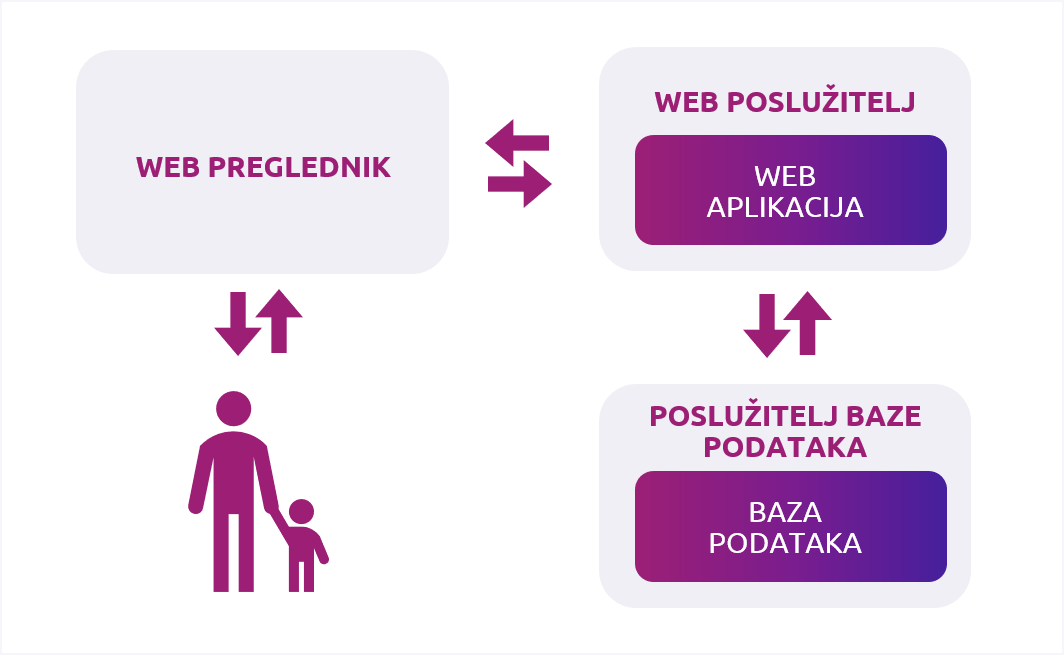
\includegraphics[scale=0.4]{slike/graf1b.PNG} %veličina slike u odnosu na originalnu datoteku i pozicija slike
			\centering
			\caption{Dijagram arhitekture projekta}
			\label{fig:arhitektura-sustava}
		\end{figure}
		
		\text	Web preglednik je program koji omogućava korisnicima pregledavanje web-stranica i multimedijskih sadržaja, te interakciju s njima. Svaki web preglednik također je i svojevrsni prevoditelj, koji programski kod otvorenih stranica interpretira u razumljivi format za korisnike. Kada korisnik koristi web aplikacije, njegovi zahtjevi šalju se putem web preglednika prema web poslužitelju. \\
		\\
		\text	Web poslužitelj glavni je dio zadužen za rad aplikacije. S njime korisnik komunicira s web aplikacijom. Ta komunikacija vrši se putem HTTP protokola (engl. \textit{Hyper Text Transfer Protokol}). Web poslužitelj također je zadužen za pokretanje web aplikacije, nakon čega joj šalje korisničke zahtjeve. \\
		\\
		\text	Web aplikacija obrađuje korisničke zahtjeve, prilikom čega pristupa bazi podataka. Obrađene podatke vraća korisniku putem poslužitelja, koji zatim navedene podatke prikazuje u web pregledniku. \\
		\\
		\text	Prilikom razvoja ovog projekta, koristili smo programski jezik Java i alat \textit{Spring Boot} za razvoj web aplikacije. Za razvoj izgleda kakav se prikazuje u web pregledniku koristili smo programski jezik Java-Script i Java-Script biblioteku \textit{React}. Razvoj projekta vršio se u razvojnom okruženju \textit{IntelliJ IDEA}.  \\
		\\
		\text	Za razvoj našeg projekta odlučili smo se ugledati na MVC [Model-Pogled-Nadglednik] (engl. \textit{Model-View-Controller}) koncept arhitekture sustava. Glavna karakteristika imenovanog koncepta jest smanjena međuovisnost korisničkog sučelja i ostatka sustava. Takav koncept omogućava lakše testiranje i daljnji razvoj sustava.
		\begin{packed_item}
			\item \textbf{Model} - Središnji dio cijelog sustava. Sadrži razrede čiji se objekti/podaci obrađuju. Izravno upravlja s podacima i pravilima aplikacije.
			\item \textbf{Pogled} - Sadrži razrede čiji objekti služe za prikaz podataka, u bilo kojem obliku.
			\item \textbf{Nadglednik} - Sadrži razrede koji upravljaju i rukuju korisničkom interakcijom s pogledom i modelom. 
		\end{packed_item}
		\text	Također smo se u našem kodu odlučili koristiti \textit{Controller-Service-Repository} uzorkom koji je dosta čest u aplikacijama koje koriste \textit{Spring Boot} alat. On se, očito iz naziva, sastoji od tri dijela:
		\begin{packed_item}
			\item \textbf{Controller} - "Najviši" dio. Služi za bilo kakvu interakciju između okoline aplikacije i njene unutarnje logike, na primjer za primanje i obradu zahtjeva poput \textit{POST} i \textit{GET}.
			\item \textbf{Service} - "Središnji" dio. Unutar njega se implementiraju sve funkcije i sva logika aplikacije. Služi za pisanje kompleksne interakcije s bazom podataka i podacima u njoj.
			\item \textbf{Repository} - "Najniži" dio. Esencijalno se radi o bazi podataka. Služi za spremanje entiteta unutar sustava. Može imati vlastite funkcije, poput \textit{Save}, ali njih može pozivati i \textit{Service}. 
		\end{packed_item}
		\clearpage
		
		
		

				
		\section{Baza podataka}
			
			\text Za potrebe našeg projekta koristili smo relacijsku bazu podataka napisanu u programskom jeziku Java, pokrenutu \textit{engine-om} H2. Prednost te vrste baze podataka jest jednostavnost modeliranja pravog svijeta na temelju relacija. Zadaća baze podataka u projektu jest pohrana, izmjena i dohvat podataka koji se zatim obrađuju. Baza podataka sastoji se od entiteta:
			\begin{packed_item}
				\item Roditelj
				\item Dijete
				\item Pedijatar
				\item Liječnik obiteljske medicine
				\item Medicinski karton
				\item Pregled
				\item Nalaz
				\item Obavijest
				\item Specijalistički pregled
				\item Preporuka o bolovanju
				\item Ispričnica
			\end{packed_item}
		
			\subsection{Opis tablica}
			

				\textbf{Roditelj} - Entitet sadržava sve podatke koje roditelj unosi prilikom registracije. Oni su: OIB, ime i prezime, datum rođenja, korisničko ime, lozinka, broj telefona, e-mail, poštanski broj, mjesto prebivališta, e-mail poslodavca te šifra liječnika. Entitet roditelj u odnosu je \textit{Many-to-One} s entitetom Liječnik obiteljske medicine preko šifre tog liječnika, u odnosu \textit{One-to-Many} sa entitetom Dijete, putem vlastitog OIB-a, te u odnosu \textit{One-to-One} s entitetom Medicinski karton, putem jedinstvenog identifikatora kartona.
				
				
				\begin{longtblr}[
					label=none,
					entry=none
					]{
						width = \textwidth,
						colspec={|X[10,l]|X[6, l]|X[20, l]|}, 
						rowhead = 1,
					} %definicija širine tablice, širine stupaca, poravnanje i broja redaka naslova tablice
					\hline \SetCell[c=3]{c}{\textbf{Parent/Roditelj}}	 \\ \hline[3pt]
					\SetCell{LightGreen}OIB & CHAR(11)	&  	Jedinstveni identifikator roditelja	\\ \hline
					nameParent	& VARCHAR &   Ime roditelja	\\ \hline 
					lastNameParent	& VARCHAR &   Prezime roditelja	\\ \hline 
					dateOfBirthParent	& DATE &  Datum rođenja roditelja 	\\ \hline 
					userNameParent	& VARCHAR &   Korisničko ime računa	\\ \hline 
					passwordParent	& VARCHAR &   Zaporka računa	\\ \hline 
					phoneNumberParent	& VARCHAR &   Broj telefona roditelja	\\ \hline 
					emailParent	& VARCHAR &   E-mail roditelja	\\ \hline 
					postalCode & INT &  Poštanski broj mjesta stanovanja \\ \hline 
					placeOfResidence & VARCHAR	&  	Mjesto stanovanja roditelja	\\ \hline 
					employerEmail	& VARCHAR &   E-mail poslodavca roditelja	\\ \hline 
					\SetCell{LightBlue}doctorId	& INT &   Identifikator L.O.M.-a roditelja	\\ \hline
					\SetCell{LightBlue}recordId	& INT &   Identifikator medicinskog kartona roditelja	\\ \hline
				\end{longtblr}
				
				\textbf{Dijete} - Entitet sadržava sve podatke koje unosi pedijatar prilikom prvog pregleda djeteta. Oni su: OIB, OIB roditelja, šifra pedijatra, ime i prezime, datum rođenja, naziv škole/vrtića te e-mail škole/vrtića. Entitet dijete u odnosu je \textit{Many-to-One} sa entitetom Roditelj, putem roditeljevog OIB-a, u odnosu \textit{Many-to-One} s entitetom Pedijatar putem pedijatrovog ID-a, te u odnosu \textit{One-to-One} s entitetom Medicinski karton, putem jedinstvenog identifikatora kartona.
				
				\begin{longtblr}[
					label=none,
					entry=none
					]{
						width = \textwidth,
						colspec={|X[11,l]|X[6, l]|X[20, l]|}, 
						rowhead = 1,
					} %definicija širine tablice, širine stupaca, poravnanje i broja redaka naslova tablice
					\hline \SetCell[c=3]{c}{\textbf{Child/Dijete}}	 \\ \hline[3pt]
					\SetCell{LightGreen}OIB & CHAR(11)	&  	Jedinstveni identifikator djeteta 	\\ \hline
					nameChild	& VARCHAR &   Ime djeteta	\\ \hline 
					lastNameChild	& VARCHAR &   Prezime djeteta	\\ \hline 
					dateOfBirthChild	& DATE &   Datum rođenja djeteta	\\ \hline 
					educationalInstitution	& VARCHAR &   Ime škole/vrtića djeteta	\\ \hline 
					emailEduInstitution & VARCHAR &  E-mail škole/vrtića \\ \hline 
					\SetCell{LightBlue} pediatricanId	& INT &   Jedinstveni identifikator pedijatra	\\ \hline 
					\SetCell{LightBlue}recordId	& INT &   Identifikator medicinskog kartona djeteta	\\ \hline
					\SetCell{LightBlue}parentOib & CHAR(11)	&  Jedinstveni identifikator roditelja	\\ \hline 
				\end{longtblr}
				
				\textbf{Pedijatar} - Entitet sadržava sve podatke koje unosi administrator prilikom registracije pedijatra u sustav. Oni su: šifra pedijatra, ime i prezime, datum rođenja, korisničko ime, lozinka, broj telefona, e-mail. Entitet pedijatar u odnosu je \textit{One-to-Many} s entitetom Dijete putem vlastite šifre.
				
				\begin{longtblr}[
					label=none,
					entry=none
					]{
						width = \textwidth,
						colspec={|X[12,l]|X[6, l]|X[20, l]|}, 
						rowhead = 1,
					} %definicija širine tablice, širine stupaca, poravnanje i broja redaka naslova tablice
					\hline \SetCell[c=3]{c}{\textbf{Pediatrician/Pedijatar}}	 \\ \hline[3pt]
					\SetCell{LightGreen}pediatricianId & INT	&  	Jedinstveni identifikator pedijatra	\\ \hline
					namePediatirican	& VARCHAR &   Ime pedijatra	\\ \hline 
					lastNamePediatirican	& VARCHAR &   Prezime pedijatra	\\ \hline 
					dateOfBirthPediatirican	& DATE &   Datum rođenja pedijatra	\\ \hline 
					userNamePediatirican	& VARCHAR &   Korisničko ime računa	\\ \hline 
					passwordPediatrician & VARCHAR &  Zaporka računa \\ \hline 
					phoneNumPediatrician	& VARCHAR &   Broj telefona pedijatra	\\ \hline 
					emailPediatrician	& VARCHAR &   E-mail pedijatra	\\ \hline
					
				\end{longtblr}
				
				\textbf{Liječnik obiteljske medicine} - Entitet sadržava sve podatke koje unosi administrator prilikom registracije LOM-a u sustav. Oni su: šifra doktora, ime i prezime, datum rođenja, korisničko ime, lozinka, broj telefona i e-mail. Entitet Liječnik obiteljske medicine u odnosu je \textit{One-to-Many} s entitetom Roditelj putem vlastite šifre.
				
				\begin{longtblr}[
					label=none,
					entry=none
					]{
						width = \textwidth,
						colspec={|X[10,l]|X[6, l]|X[20, l]|}, 
						rowhead = 1,
					} %definicija širine tablice, širine stupaca, poravnanje i broja redaka naslova tablice
					\hline \SetCell[c=3]{c}{\textbf{Doctor/Liječnik obiteljske medicine}}	 \\ \hline[3pt]
					\SetCell{LightGreen}doctorId & INT	&  	Jedinstveni identifikator liječnika	\\ \hline
					nameDoctor	& VARCHAR &   Ime liječnika	\\ \hline 
					lastNameDoctor	& VARCHAR &   Prezime liječnika	\\ \hline 
					dateOfBirthDoctor	& DATE &   Datum rođenja liječnika	\\ \hline 
					userNameDoctor	& VARCHAR &   Korisničko ime računa	\\ \hline 
					passwordDoctor & VARCHAR &  Zaporka računa \\ \hline 
					phoneNumDoctor	& VARCHAR &   Broj telefona liječnika	\\ \hline 
					emailDoctor	& VARCHAR &   E-mail liječnika	\\ \hline
					
				\end{longtblr}
				
				\textbf{Medicinski karton} - Entitet sadržava podatke za opis medicinskog kartona pojedinog pacijenta (roditelj/dijete). Oni su: šifra kartona, OIB, trenutna dijagnoza i popis alergija. Entitet Medicinski karton u odnosu je \textit{One-to-One} s entitetom Roditelj i s entitetom Dijete, putem vlastitog jedinstvenog identifikatora, te u odnosima \textit{One-to-Many} s entitetima Nalaz i Pregled.  
				
				\begin{longtblr}[
					label=none,
					entry=none
					]{
						width = \textwidth,
						colspec={|X[8,l]|X[6, l]|X[20, l]|}, 
						rowhead = 1,
					} %definicija širine tablice, širine stupaca, poravnanje i broja redaka naslova tablice
					\hline \SetCell[c=3]{c}{\textbf{MedicalRecord/Medicinski karton}}	 \\ \hline[3pt]
					\SetCell{LightGreen}redordId & INT	&  	Jedinstveni identifikator kartona	\\ \hline
					currentDiagnosis & VARCHAR &  Aktivna ili zadnja dijagnoza djeteta \\ \hline 
					allergyList & VARCHAR	&  	Popis alergija djeteta	\\ \hline
				\end{longtblr}
				
				\textbf{Pregled} - Entitet sadržava podatke pregleda kojeg održava pedijatar ili LOM. Oni su: šifra pregleda, šifra kartona kojem pripada, dijagnoza i datum pregleda. Entitet Pregled u odnosu je \textit{Many-to-One} s entitetom Medicinski karton.
				
				\begin{longtblr}[
					label=none,
					entry=none
					]{
						width = \textwidth,
						colspec={|X[9,l]|X[6, l]|X[20, l]|}, 
						rowhead = 1,
					} %definicija širine tablice, širine stupaca, poravnanje i broja redaka naslova tablice
					\hline \SetCell[c=3]{c}{\textbf{Examination/Pregled}}	 \\ \hline[3pt]
					\SetCell{LightGreen}examinationId & INT	&  	Jedinstveni identifikator pregleda	\\ \hline
					\SetCell{LightBlue}recordId	& INT &  Jedinstveni identifikator kartona 	\\ \hline 
					diagnosis & VARCHAR &  Opis dijagnoze  \\ \hline 
					dateOfExamination & DATE	&  	Datum pregleda	\\ \hline
				\end{longtblr}
				
				\textbf{Nalaz} - Entitet sadržava podatke koji opisuju nalaz dobiven prilikom privatnog pregleda, kojeg \textit{uploada} roditelj. Oni su: šifra nalaza, šifra kartona, datum nalaza, podaci nalaza. Entitet Nalaz u odnosu je \textit{Many-to-One} s entitetom Medicinski karton.
				
				\begin{longtblr}[
					label=none,
					entry=none
					]{
						width = \textwidth,
						colspec={|X[9,l]|X[6, l]|X[20, l]|}, 
						rowhead = 1,
					} %definicija širine tablice, širine stupaca, poravnanje i broja redaka naslova tablice
					\hline \SetCell[c=3]{c}{\textbf{MedicalReport/Nalaz}}	 \\ \hline[3pt]
					\SetCell{LightGreen}reportId & INT	&  	Jedinstveni identifikator nalaza	\\ \hline
					\SetCell{LightBlue}recordId	& INT &  Jedinstveni identifikator kartona 	\\ \hline 
					reportInformation & VARCHAR &  Podaci iz nalaza  \\ \hline 
					dateOfReport & DATE	&  	Datum pregleda	\\ \hline
				\end{longtblr}
				
				\textbf{Obavijest} - Entitet sadržava podatke koji opisuju obavijest poslanu roditelju, koju piše liječnik/pedijatar. Oni su: šifra obavijesti, OIB roditelja, OIB djeteta, naslov i tekst obavijesti. Entitet Obavijest u odnosu je \textit{Many-to-One} s entitetima Roditelj i Dijete.
				
				\begin{longtblr}[
					label=none,
					entry=none
					]{
						width = \textwidth,
						colspec={|X[11,l]|X[6, l]|X[20, l]|}, 
						rowhead = 1,
					} %definicija širine tablice, širine stupaca, poravnanje i broja redaka naslova tablice
					\hline \SetCell[c=3]{c}{\textbf{Notification/Obavijest}}	 \\ \hline[3pt]
					\SetCell{LightGreen}notificationId & INT	&  	Jedinstveni identifikator obavijesti	\\ \hline
					\SetCell{LightBlue}parentOib	& CHAR(11) &  Jedinstveni identifikator roditelja 	\\ \hline 
					\SetCell{LightBlue}childOib	& CHAR(11) &  Jedinstveni identifikator djeteta	\\ \hline 
					notificationInformation & VARCHAR &  Podaci obavijesti  \\ \hline 
					notificationTitle & VARCHAR &  Naslov obavijesti  \\ \hline 
				\end{longtblr}
				
				\textbf{Specijalistički pregled} - Entitet sadržava podatke koji opisuju specijalistički pregled na kojeg liječnik/pedijatar prijavljuje pacijenta. Oni su: šifra pregleda, šifra pacijenta, naziv pregleda, moguće lokacije pregleda. Entitet Spec. pregled u odnosu je \textit{Many-to-One} s entitetom Medicinski karton, preko čega mu pristupaju entiteti Roditelj i Dijete.
				
				\begin{longtblr}[
					label=none,
					entry=none
					]{
						width = \textwidth,
						colspec={|X[9,l]|X[6, l]|X[20, l]|}, 
						rowhead = 1,
					} %definicija širine tablice, širine stupaca, poravnanje i broja redaka naslova tablice
					\hline \SetCell[c=3]{c}{\textbf{SpecialistExamination/Specijalistički pregled}}	 \\ \hline[3pt]
					\SetCell{LightGreen}examId & INT	&  	Jedinstveni identifikator pregleda	\\ \hline
					\SetCell{LightBlue}recordId	& INT &  Jedinstveni identifikator kartona	\\ \hline 
					examTitle & VARCHAR &  Naziv pregleda  \\ \hline 
					examLocations & VARCHAR	&  	Moguće lokacije pregleda	\\ \hline
				\end{longtblr}
				
				\textbf{Preporuka o bolovanju} - Entitet sadržava podatke o bolovanju kojeg pedijatar preporučuje za roditelja djeteta. Oni su: šifra preporuke, šifra liječnika obiteljske medicine, opis razloga za bolovanje i trajanja, te email poslodavca. Entitet Preporuka o bolovanju u odnosu je \textit{Many-to-One} s entitetom Liječnik obiteljske medicine.
				
				\begin{longtblr}[
					label=none,
					entry=none
					]{
						width = \textwidth,
						colspec={|X[9,l]|X[6, l]|X[20, l]|}, 
						rowhead = 1,
					} %definicija širine tablice, širine stupaca, poravnanje i broja redaka naslova tablice
					\hline \SetCell[c=3]{c}{\textbf{SickLeaveRecommendation/Preporuka o bolovanju}}	 \\ \hline[3pt]
					\SetCell{LightGreen}recommendationId & INT	&  	Jedinstveni identifikator preporuke	\\ \hline
					\SetCell{LightBlue}doctorId	& INT &  Jedinstveni identifikator liječnika	\\ \hline 
					recData & VARCHAR &  Sadržaj preporuke  \\ \hline
					employerEmail & VARCHAR &  email poslodavca kojem se šalje doznaka  \\ \hline
				\end{longtblr}
				
				\textbf{Ispričnica} - Entitet sadržava podatke o ispričnici koju pedijatar piše za dijete. Oni su: šifra ispričnice, OIB djeteta, opis razloga za ispričnicom i trajanja. Entitet Ispričnica u odnosu je \textit{Many-to-One} s entitetom Dijete.
				
				\begin{longtblr}[
					label=none,
					entry=none
					]{
						width = \textwidth,
						colspec={|X[9,l]|X[6, l]|X[20, l]|}, 
						rowhead = 1,
					} %definicija širine tablice, širine stupaca, poravnanje i broja redaka naslova tablice
					\hline \SetCell[c=3]{c}{\textbf{SickNote/Ispričnica}}	 \\ \hline[3pt]
					\SetCell{LightGreen}sicknoteId & INT	&  	Jedinstveni identifikator ispričnice	\\ \hline
					\SetCell{LightBlue}childOib	& CHAR(11) &  Jedinstveni identifikator djeteta	\\ \hline 
					noteData & VARCHAR &  Sadržaj ispričnice  \\ \hline
				\end{longtblr}
			\subsection{Dijagrami baze podataka}
				%unos slike
				\begin{figure}[H]
					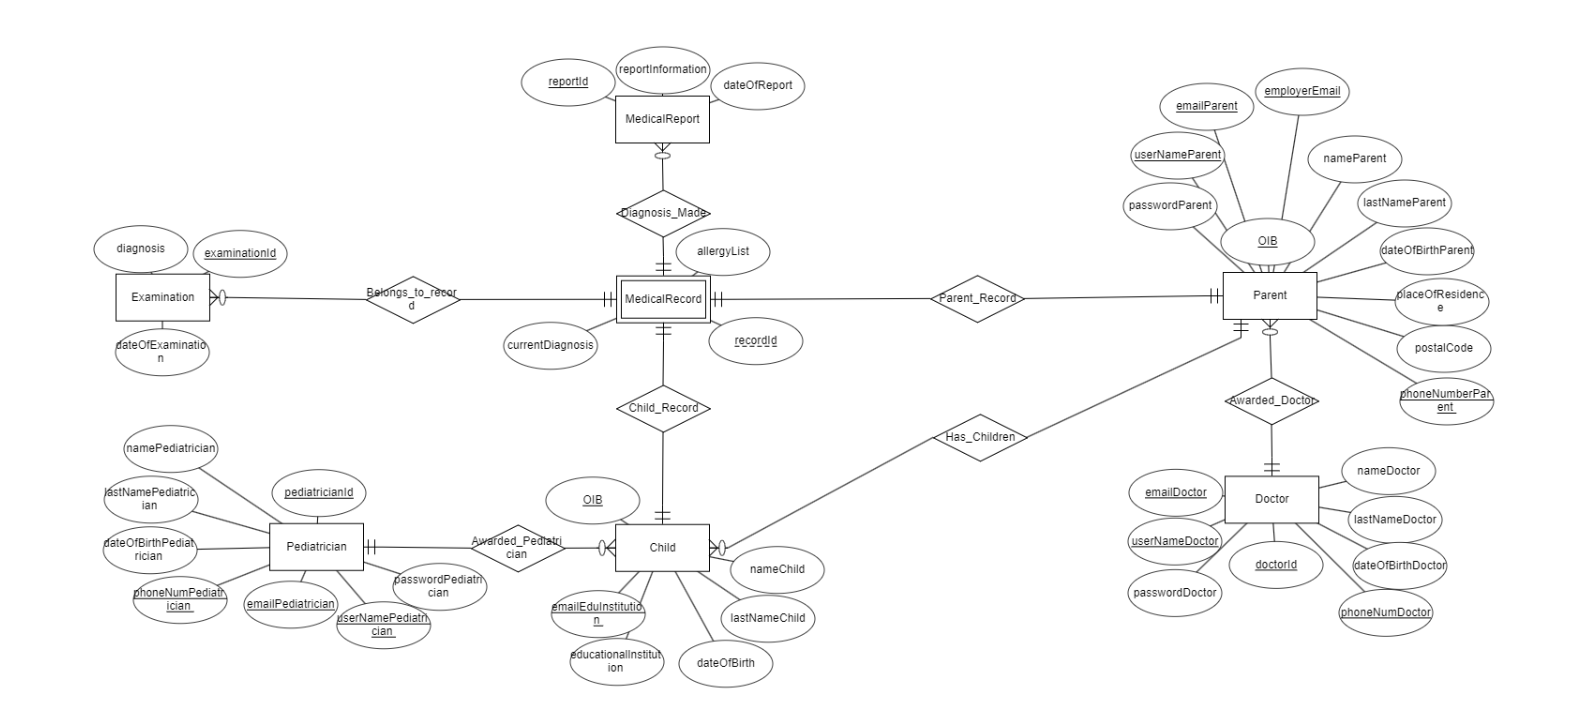
\includegraphics[scale=0.1]{dijagrami/ozdraviER.PNG} %veličina slike u odnosu na originalnu datoteku i pozicija slike
					\centering
					\caption{Dijagram arhitekture baze podataka}
					\label{fig:arhitektura-baze1}
				\end{figure}
				
				%unos slike
				\begin{figure}[H]
					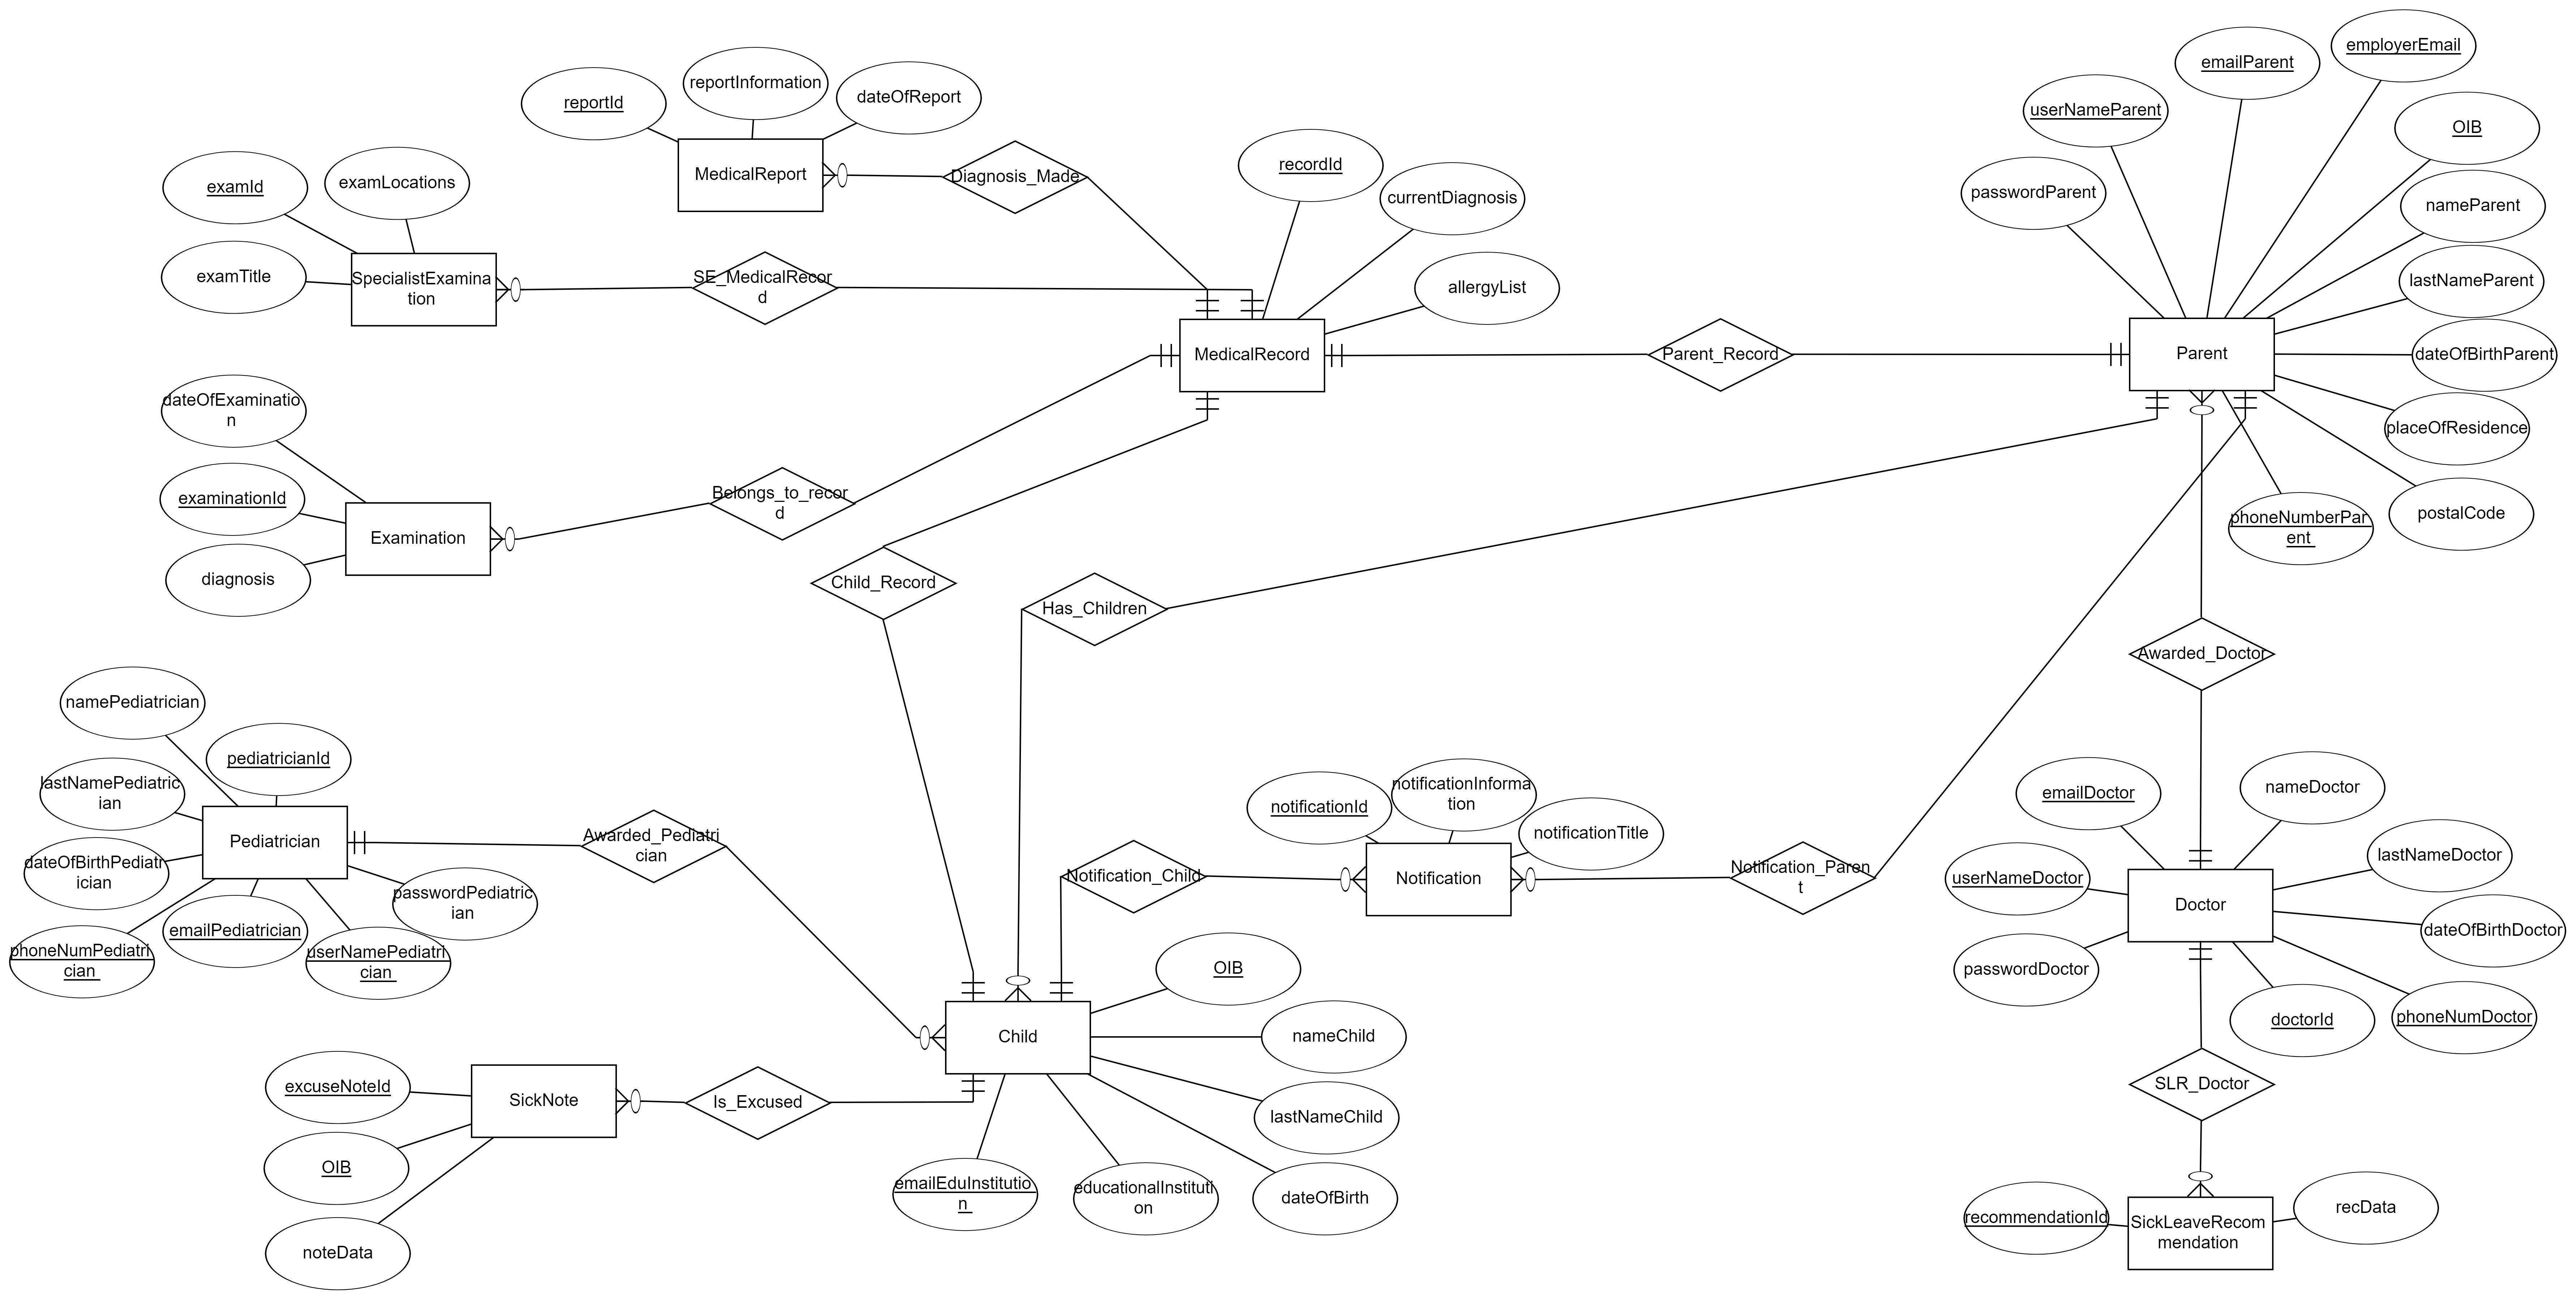
\includegraphics[scale=0.07]{dijagrami/ozdraviREL.PNG} %veličina slike u odnosu na originalnu datoteku i pozicija slike
					\centering
					\caption{Dijagram arhitekture baze podataka}
					\label{fig:arhitektura-baze2}
				\end{figure}
				\clearpage
			\eject
			
		\section{Dijagram razreda}
		
			\text Na sljedećim slikama prikazani su dijagrami razreda ovog projekta. Zbog lakšeg snalaženja, razredi su raspodijeljeni na nekoliko dijagrama.\\
			Postoje četiri razreda koji označavaju osobu: liječnik obiteljske medicine (Doctor), pedijatar (Pediatrician), roditelj (Parent) i njegovo dijete (Child). Razred Parent predstavlja roditelja koji se registrira u sustav te povezuje svoju djecu radi komunikacije s pedijatrom i liječnikom. Razred Doctor predstavlja liječnika obiteljske medicine kojeg registrira administrator i ima komunikaciju s roditeljem u vezi bolovanja, te ostalim zadaćama liječnika i pacijenta. Razred Pediatrician predstavlja pedijatra koji je zadužen za liječenje djeteta i izdavanje ispričnica i medicinskih dokumentacija. Razred Child predstavlja dijete registriranog roditelja koje se liječi kod pedijatra. Za dijete i roditelja kao pacijente vežu se tri razreda koji označavaju vrstu medicinske dokumentacije: medicinski kartoni (MedicalRecord), pregledi (Examination), specijalistički pregledi (SpecialistExamination) i nalazi (MedicalReport). Pregledi i nalazi su s djetetom povezani preko medicinskog kartona. Liječnik je povezan s roditeljem, a pedijatar je povezan s roditeljem preko djeteta. Razredi RegistrationRequest i LoginRequest služe za registraciju i prijavu korisnika u sustav.
				 
			
			%unos slike
			\begin{figure}[H]
				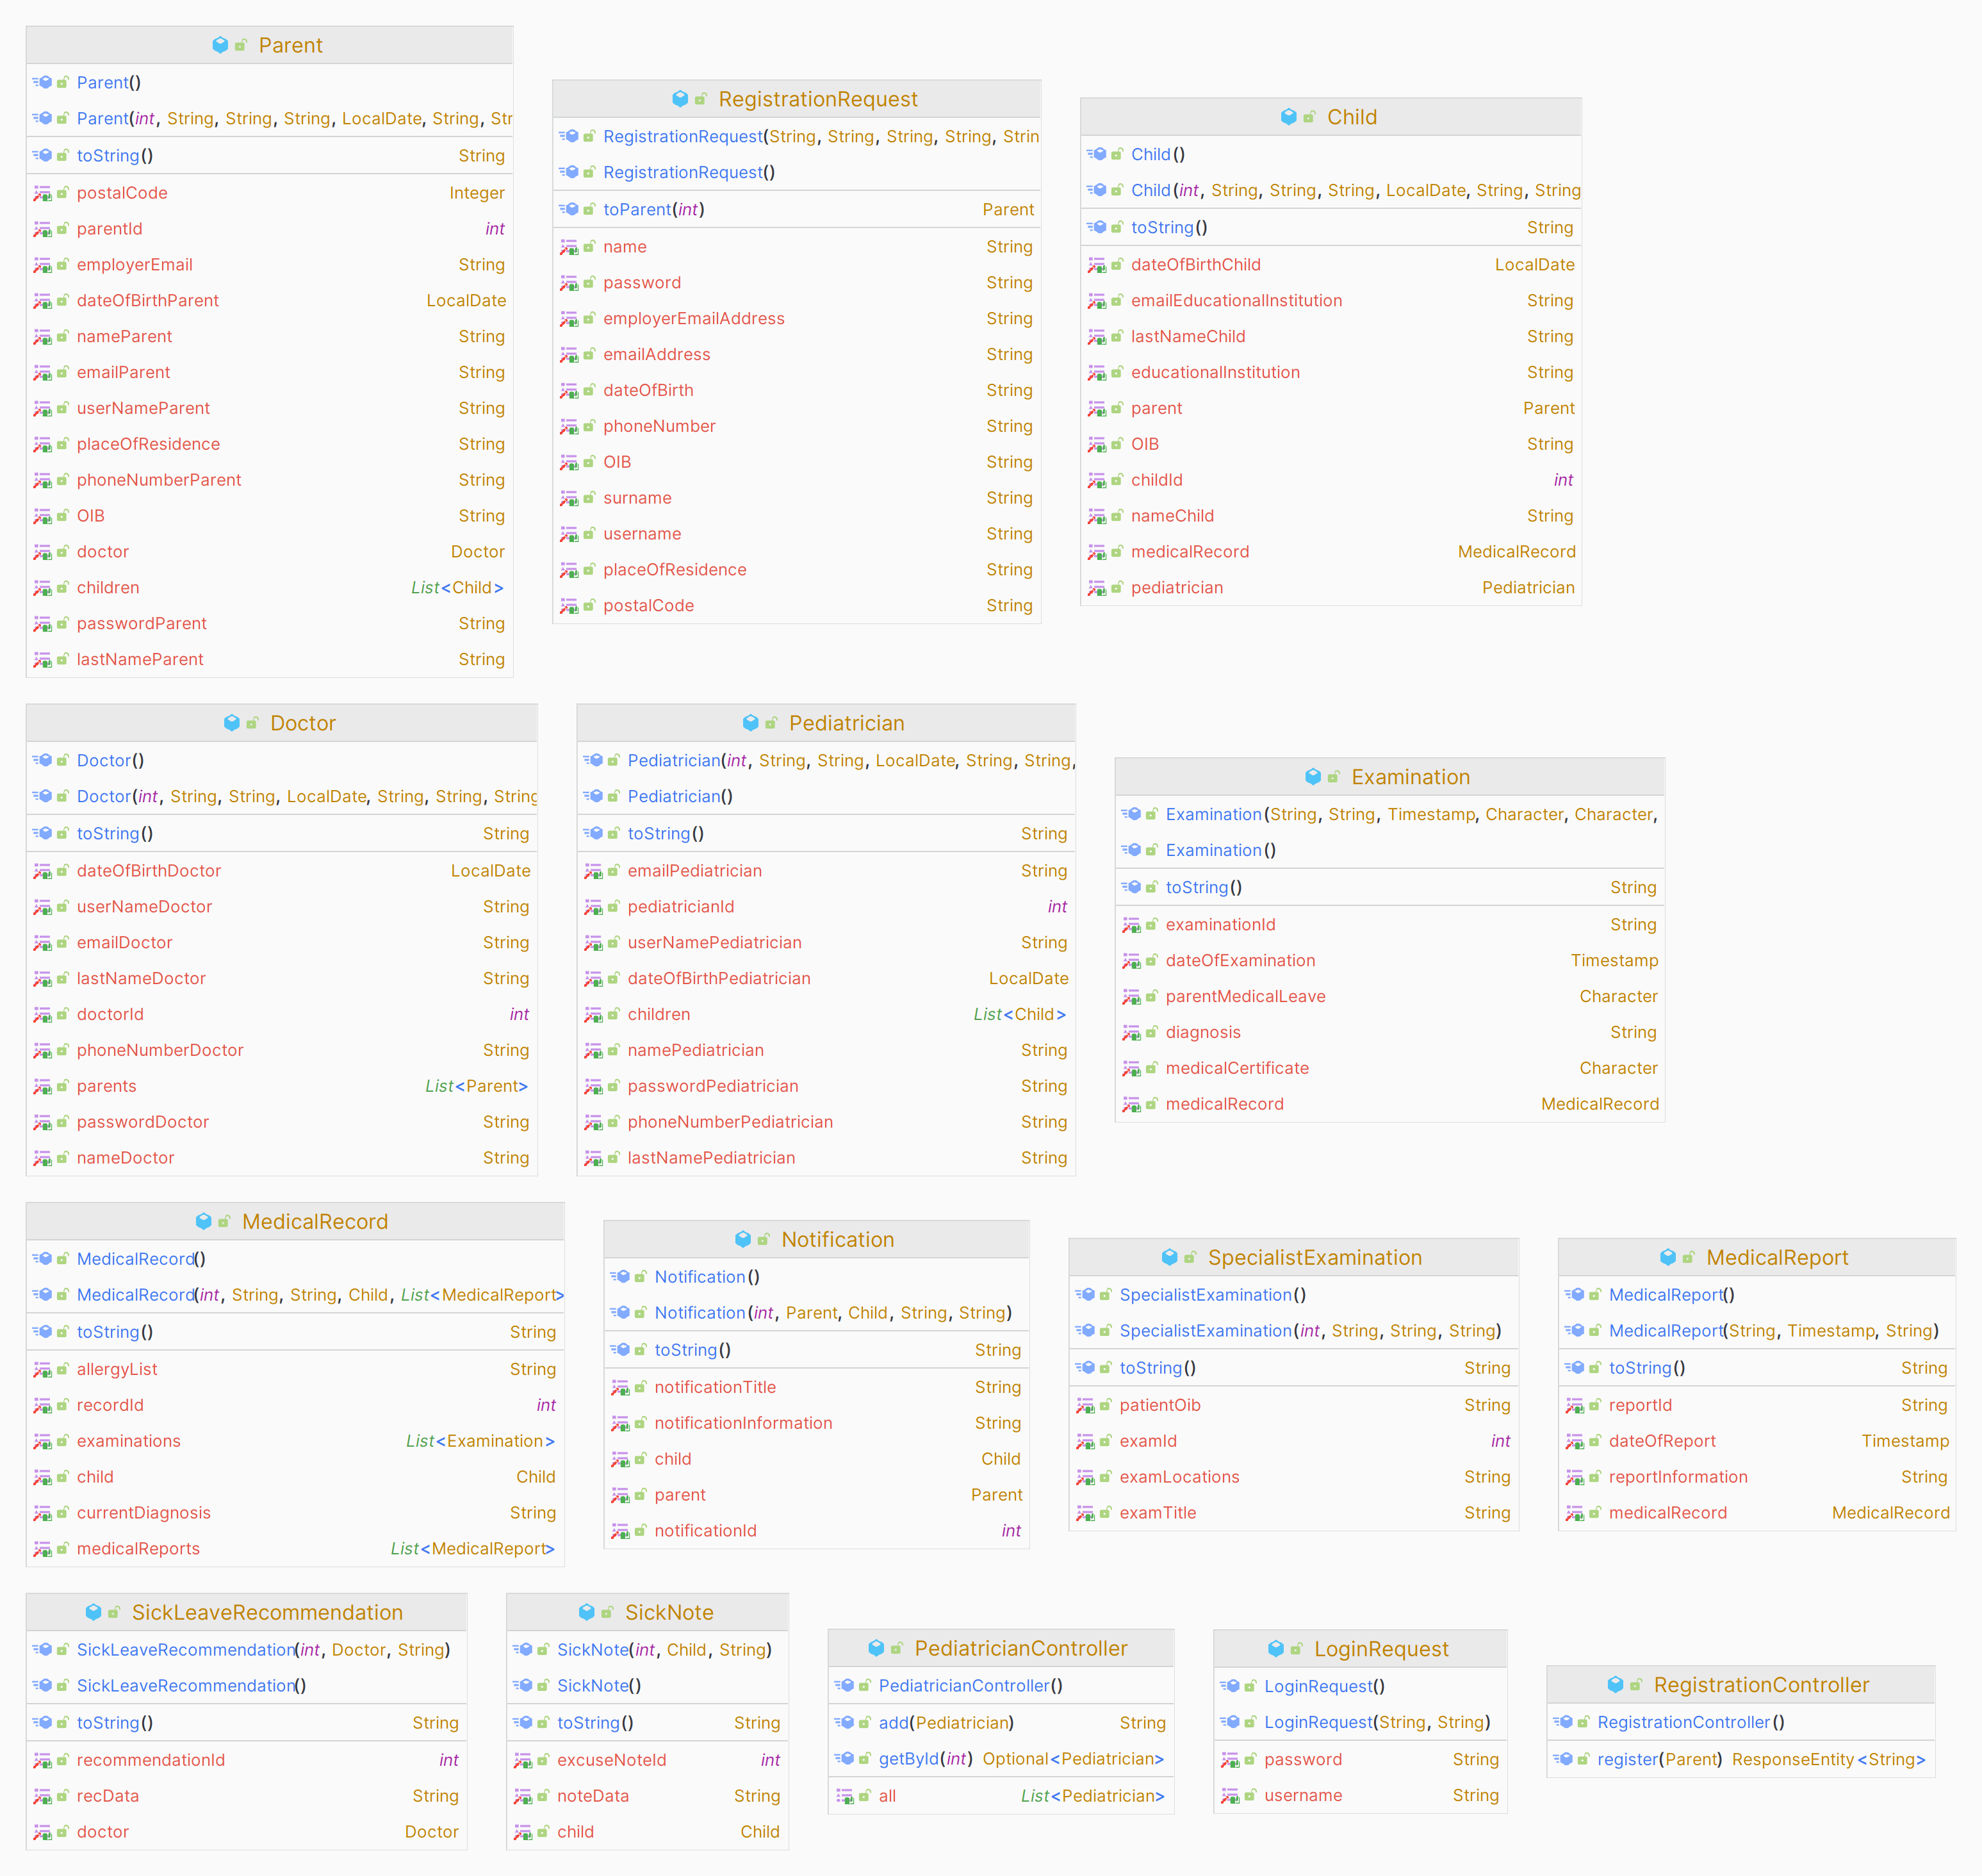
\includegraphics[scale=0.15]{dijagrami/dijraz1.PNG} %veličina slike u odnosu na originalnu datoteku i pozicija slike
				\centering
				\caption{Dijagram razreda 1}
				\label{fig:dijraz1}
			\end{figure}
			\clearpage
			\text Postoje tri razreda koji služe kao kontroleri za manipulaciju objekta i njihovo obrađivanje u bazi podataka za liječnika, pedijatra i roditelja. To su DoctorController, PediatricianController i ParentController. Postoje dva razreda RegistrationController i LoginController koji služe za rukovanje registracijama i prijavama korisnika. Za prijenos podataka između controllera i baze podataka postoje sučelja DoctorService, PediatricianService i ParentService te razredi DoctorServiceImpl, PediatricianServiceImpl i ParentServiceImpl koji implementiraju metode iz tih sučelja i osiguravaju prijenos podataka s bazom podataka preko tri sučelja koji predstavljaju repozitorije: DoctorRepository, PediatricianRepository i ParentRepository.
			%unos slike
			\begin{figure}[H]
				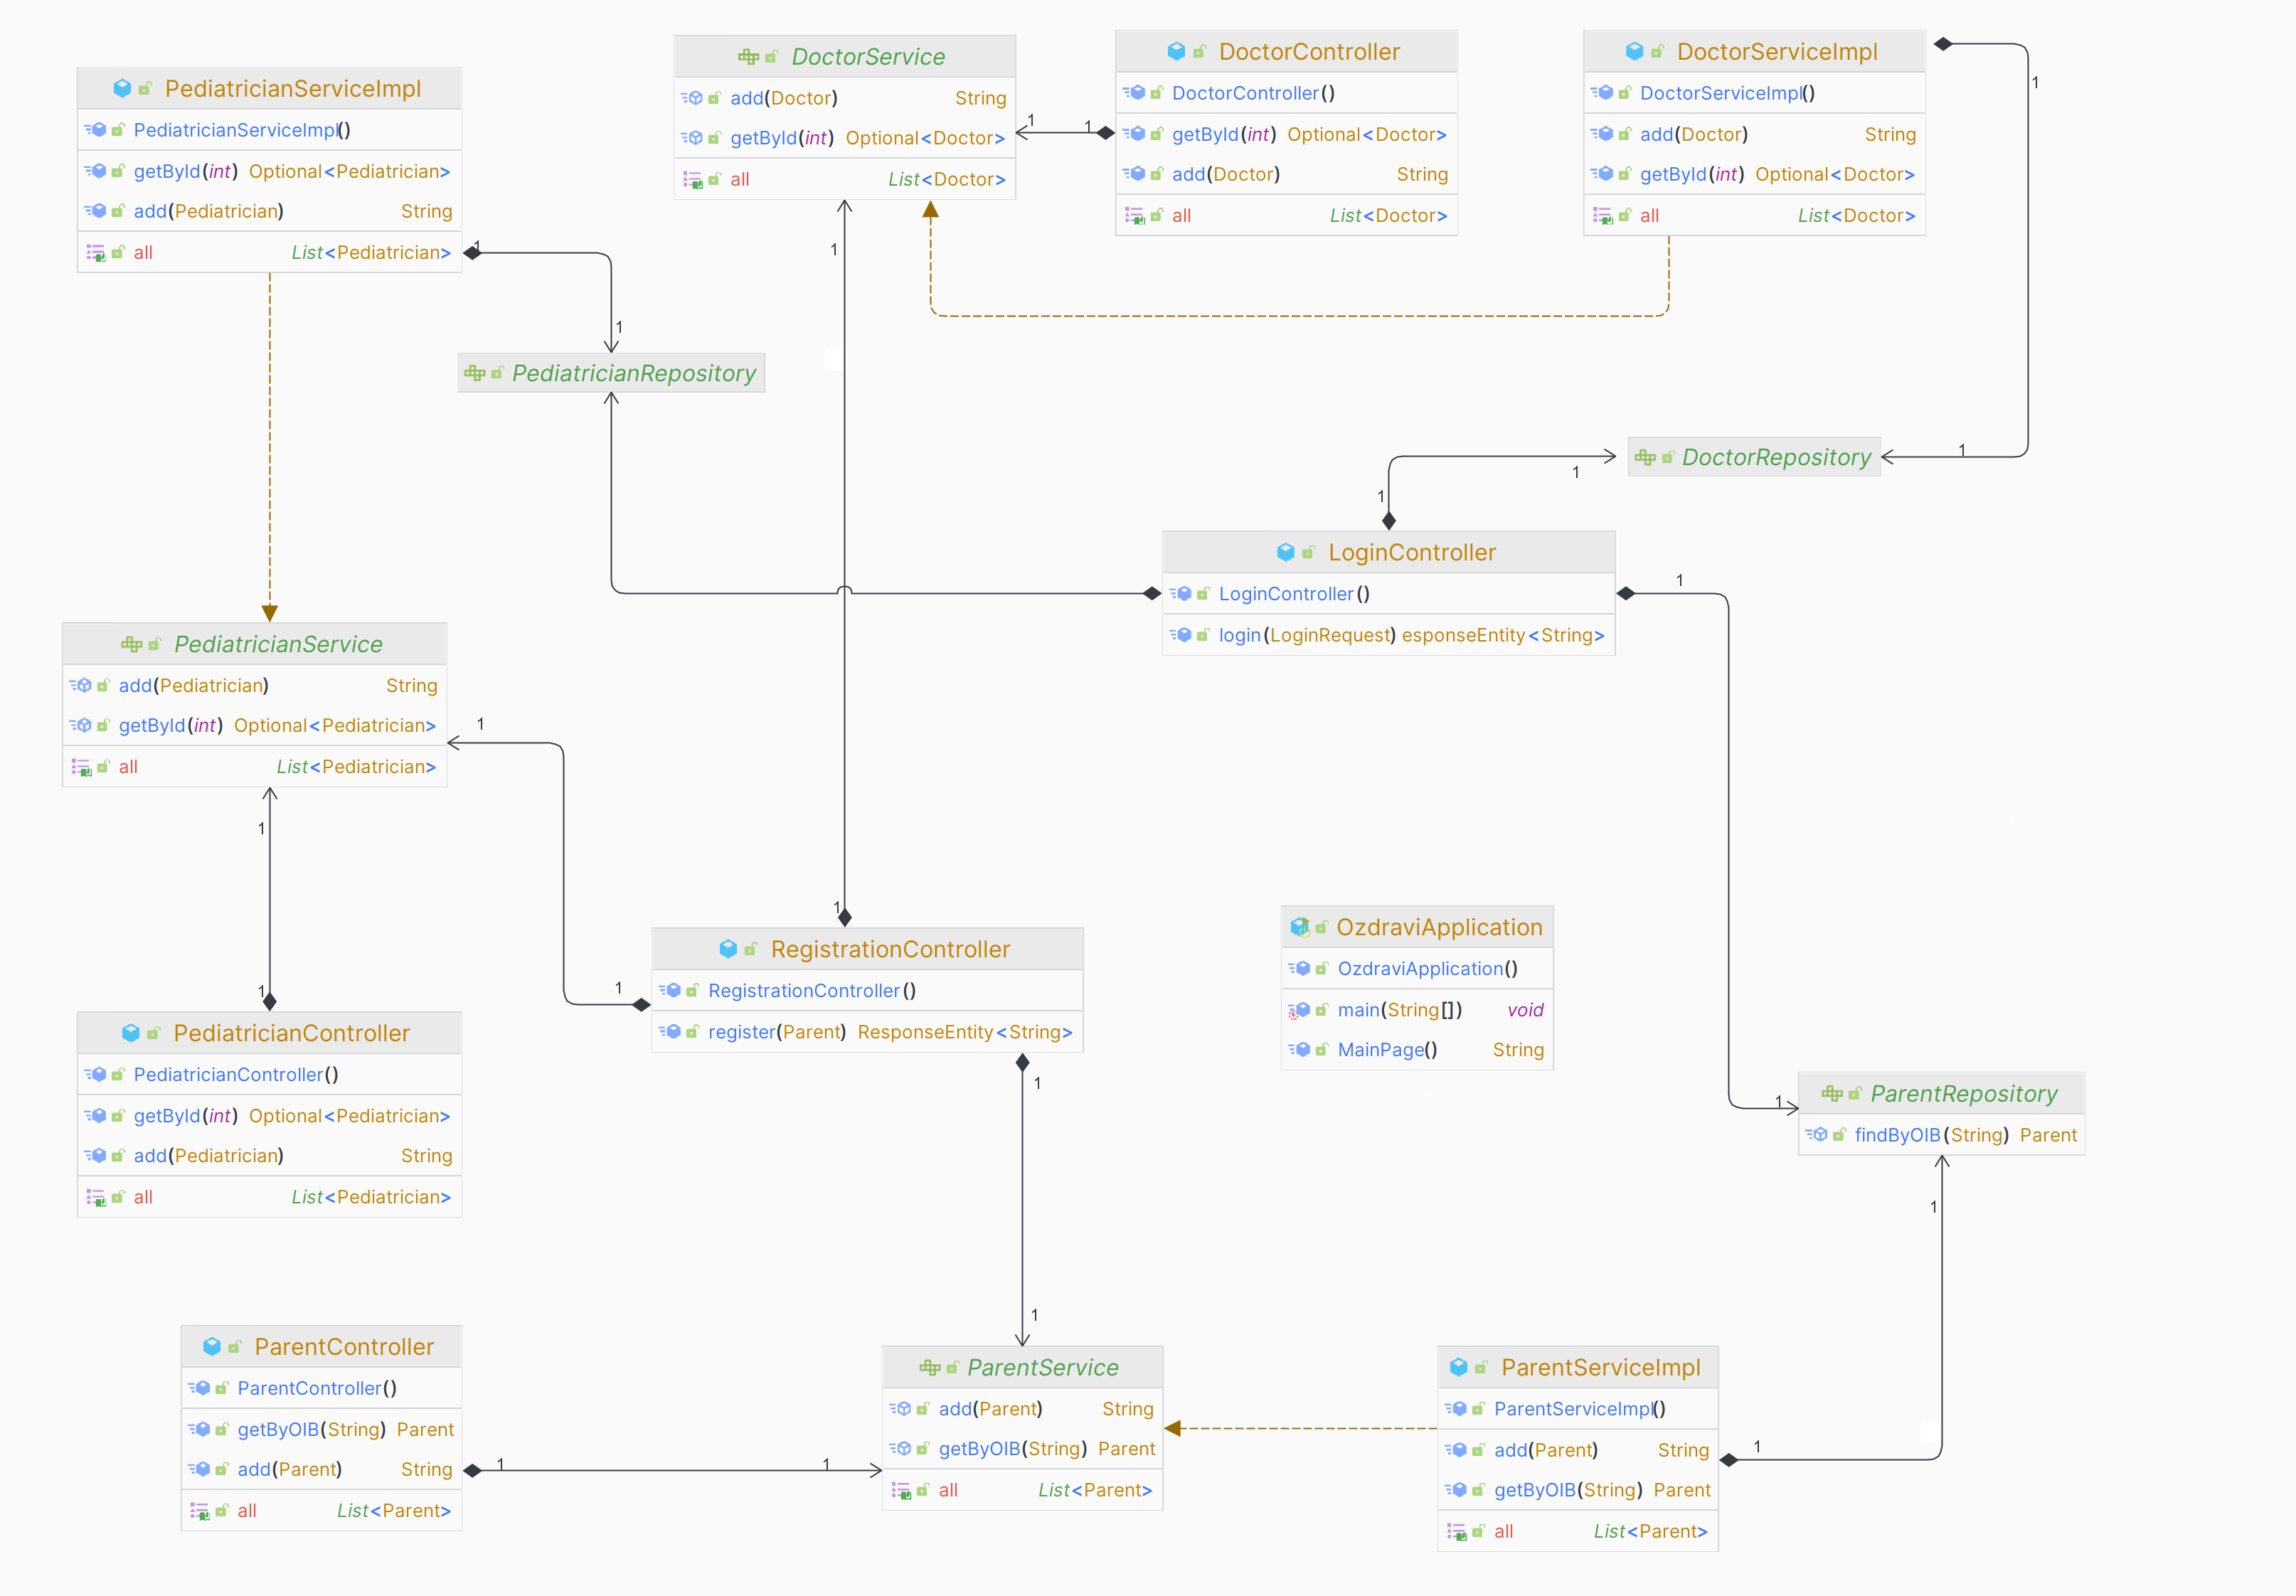
\includegraphics[scale=0.225]{dijagrami/dijraz2.PNG} %veličina slike u odnosu na originalnu datoteku i pozicija slike
				\centering
				\caption{Dijagram razreda 2}
				\label{fig:dijraz2}
			\end{figure} 
			
			%unos slike
			\begin{figure}[H]
				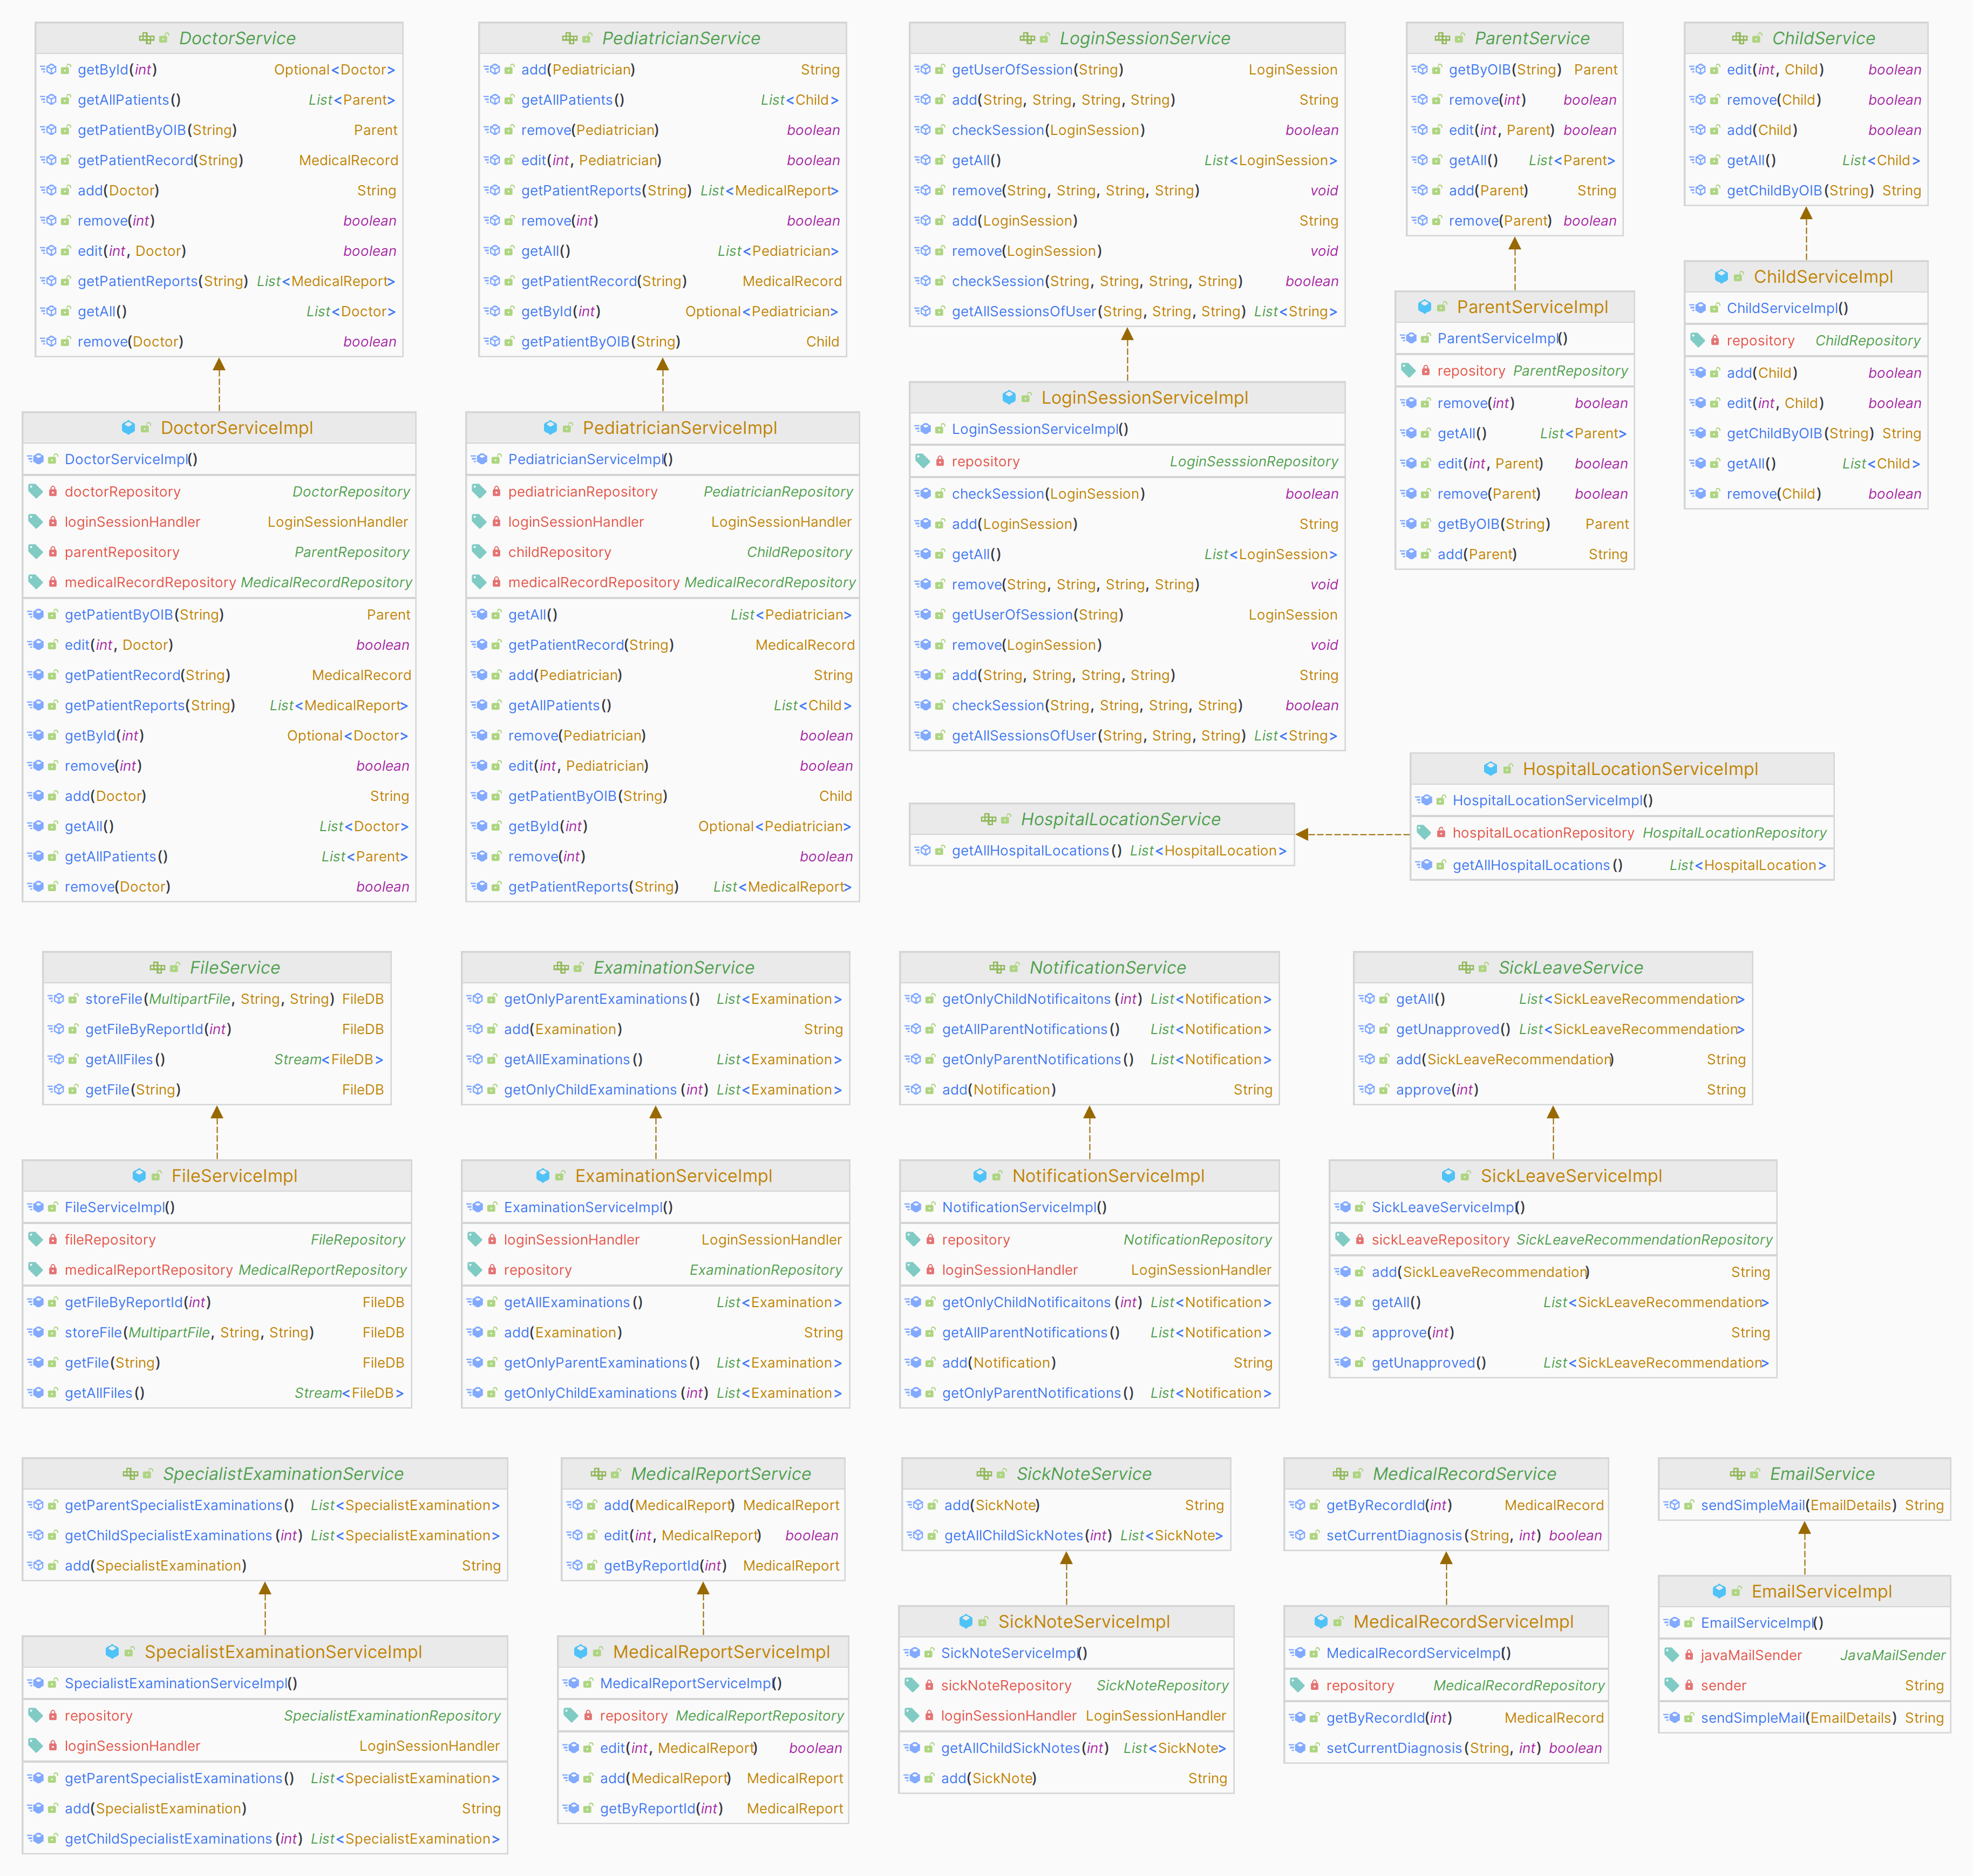
\includegraphics[scale=0.225]{dijagrami/dijraz3.PNG} %veličina slike u odnosu na originalnu datoteku i pozicija slike
				\centering
				\caption{Dijagram razreda 3}
				\label{fig:dijraz3}
			\end{figure}
			
			\textbf{\textit{dio 2. revizije}}\\			
			
			\textit{Prilikom druge predaje projekta dijagram razreda i opisi moraju odgovarati stvarnom stanju implementacije}
			
			
			
			\eject
		
		\section{Dijagram stanja}
			
			\text Dijagrami stanja pripadaju ponašajnim dijagramima u UML-u. Služe za opis diskretnih stanja sustava i prijelaza između istih. Na slici 4.7 prikazan je dijagram stanja za liječnika obiteljske medicine. Nakon prijave LOM-u se prikazuje popis njegovih pacijenata. Uz taj popis, ima opcije za prikaz preporuka za bolovanje koje je primio od raznih pedijatara, te opcija za unos novog pacijenta pomoću OIB-a istog. Uz svakog pacijenta u popisu ima opciju za otvaranje profila tog pacijenta. Nakon otvaranja profila, prvo se prikazuju osobni podaci pacijenta. Uz to, LOM ima opcije za prikaz liječničkog kartona, za unos novog pregleda odabranom pacijentu, za zakazivanje specijalističkog pregleda odabranom pacijentu, te za prikaz svih \textit{uploadanih} privatnih nalaza tog pacijenta. Svaki od tih nalaza moguće je pojedinačno otvoriti, te na svaki poslati povratnu informaciju. 
			
			%unos slike
			\begin{figure}[H]
				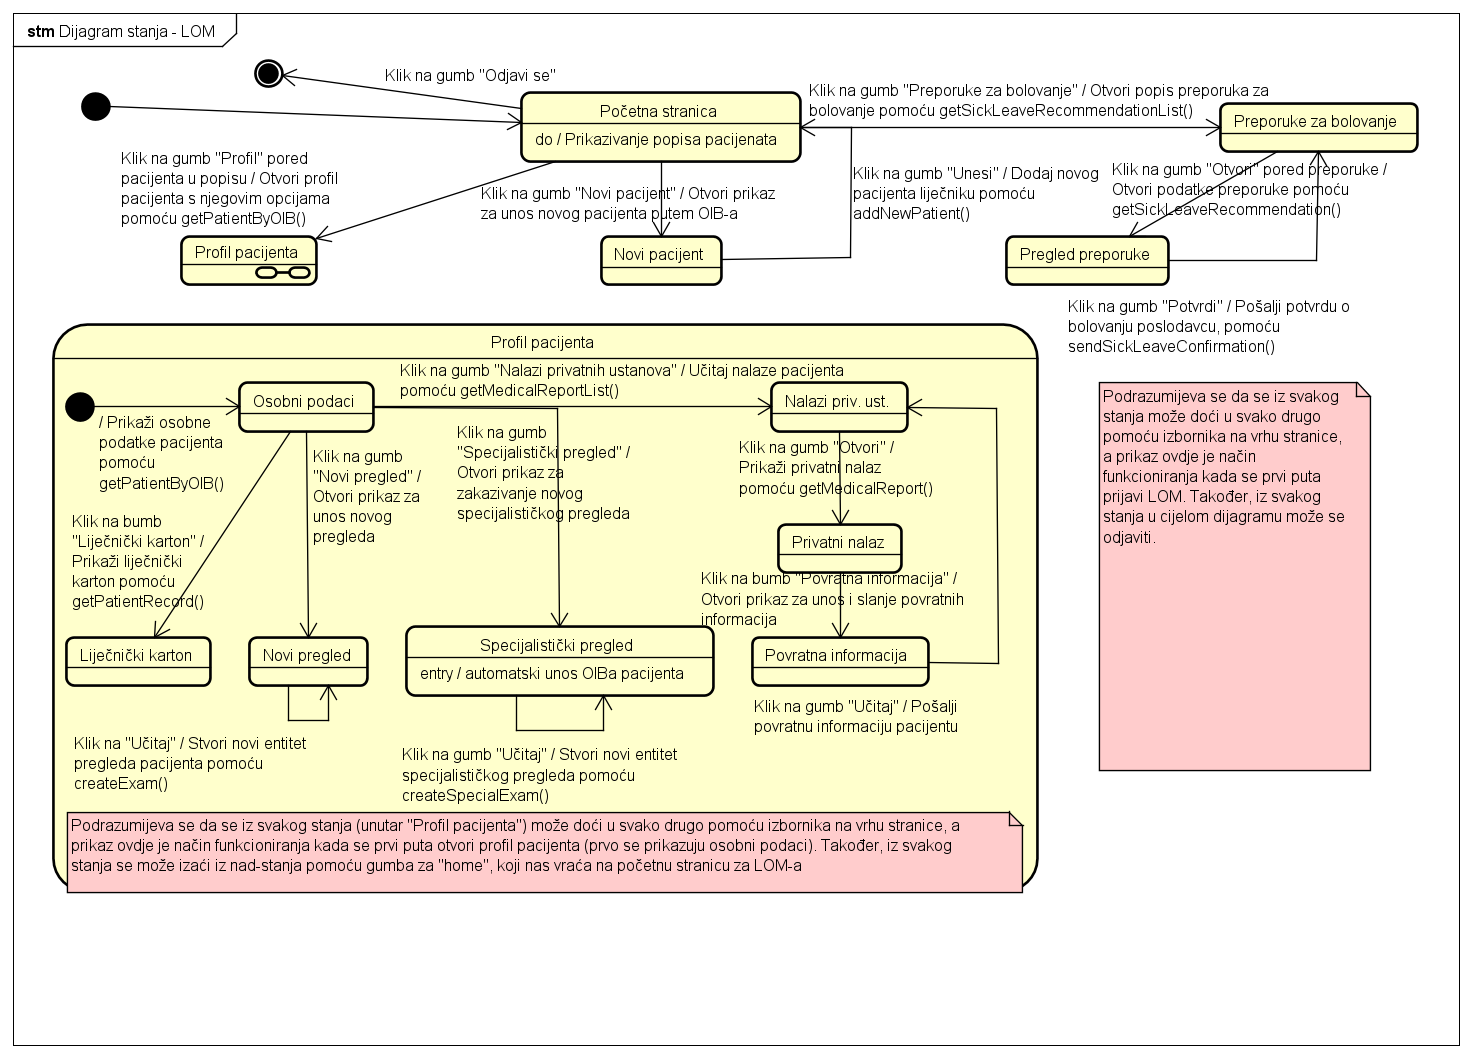
\includegraphics[scale=0.4]{dijagrami/dijstanj1.PNG} %veličina slike u odnosu na originalnu datoteku i pozicija slike
				\centering
				\caption{Dijagram stanja}
				\label{fig:dijstanj1}
			\end{figure}
			
			\eject 
		
		\section{Dijagram aktivnosti}
			
			\text Dijagrami aktivnosti prikazuju radni tok aktivnosti koje se obavljaju, korak po korak, unutar nekog sustava. Dakle, modelira se ponašanje nizom akcija. Izričit je naglasak na jednostavnosti i čitljivosti. Na slici 4.8 prikazan je dijagram aktivnosti pedijatra, web aplikacije i baze podataka prilikom generiranja ispričnice za pacijenta. Pedijatar se prijavljuje u sustav. Potom odabire pacijenta iz liste, te pritišće opciju "Generiraj ispričnicu". Web aplikacija otvara prikaz s unesenim osobnim podacima pacijenta, te poljima za unos podataka o ispričnici/bolesti. Nakon što ih pedijatar unese, stvara se entitet ispričnice, koji se šalje obrazovnoj ustanovi i sprema u bazu podataka.
			
			%unos slike
			\begin{figure}[H]
				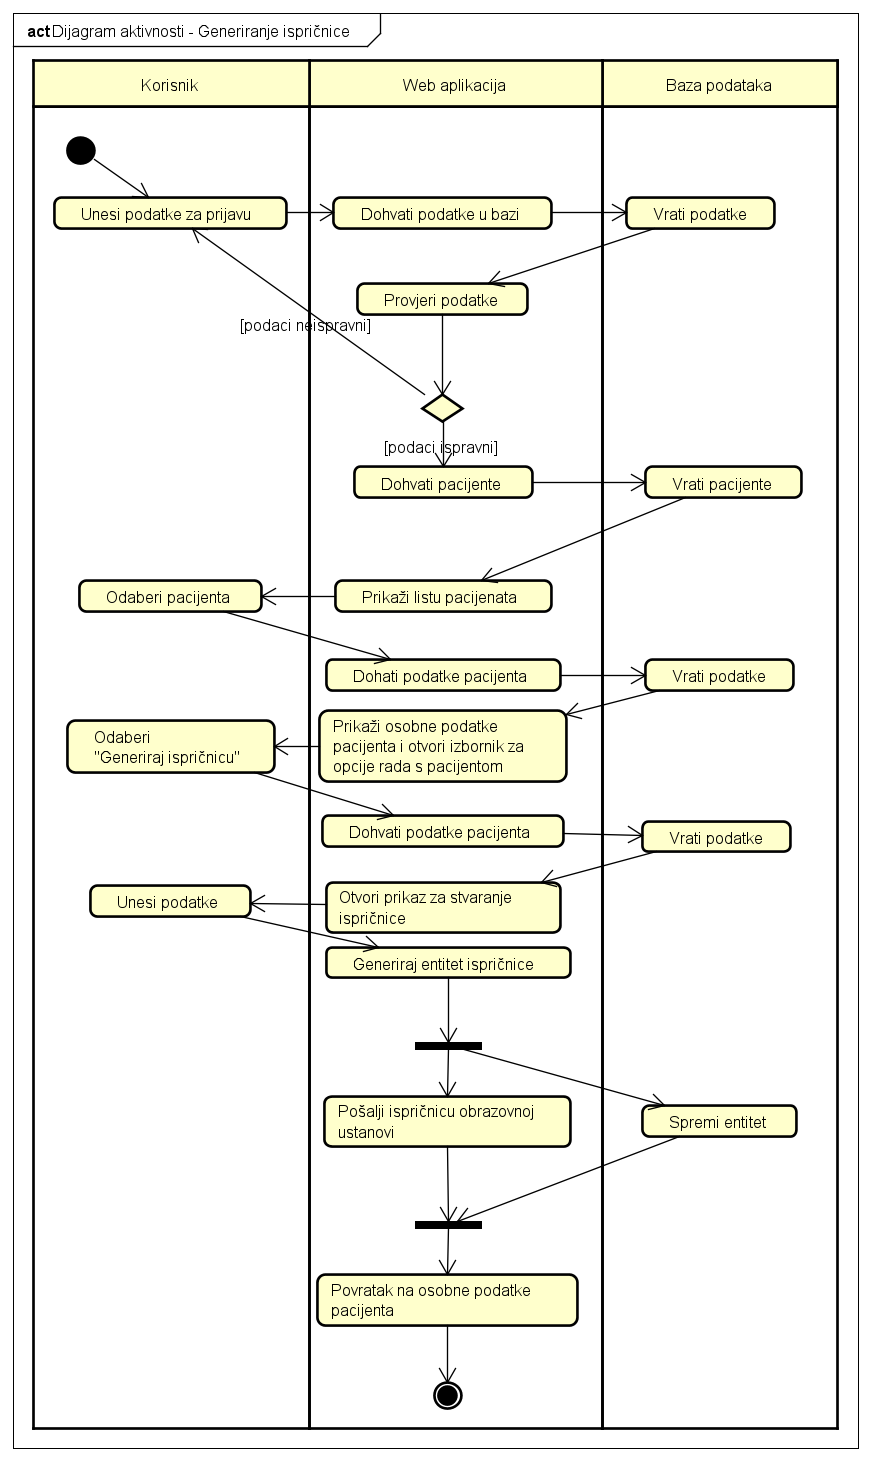
\includegraphics[scale=0.5]{dijagrami/dijakt1.PNG} %veličina slike u odnosu na originalnu datoteku i pozicija slike
				\centering
				\caption{Dijagram aktivnosti}
				\label{fig:dijakt1}
			\end{figure}
			
			\eject
		\section{Dijagram komponenti}
			\text Dijagram komponenti strukturni je i statički UML dijagram koji služi za specifikaciju arhitekture programske potpore. Vrlo je koristan za prikaz organizacije i međuovisnosti unutar građe sustava. Na slici 4.9 nalazi se dijagram komponenti koji opisuje strukturu naše aplikacije. Korisnik ima interakciju s \textit{frontend} dijelom aplikacije, unutar kojeg se nalazi vizualno sučelje \textit{React-view}. Ondje se nalaze dva sučelja za interakciju s aplikacijom. Sučelje za dohvat HTML, CSS i JavaScript datoteka poslužuje \textit{frontend} dio aplikacije i omogućuje njegov rad. Router komponenta odgovara na URL upite, te kao odgovor šalje različite React/JS datoteke. Te datoteke grupirane su radi jednostavnosti u logičke cjeline, koje su nazvane prema glavnim prikazima u aplikaciji, te po korisnicima iste. Sve JavaScript datoteke ovise o React biblioteci, jer iz nje dohvaćaju gotove komponente.
			Drugo sučelje služi za prijenos JSON podataka. REST API poslužuje te podatke. Svi podaci unutar aplikacije nalaze se u H2 bazi podataka. Ona je putem sučelja povezana s grupom komponenata Repositories, koje služe kao svojevrsni most između aplikacije i baze podataka. Services grupa komponenata vuče podatke iz repozitorija, te ih šalje upravljačima.
			%unos slike
			\begin{figure}[H]
				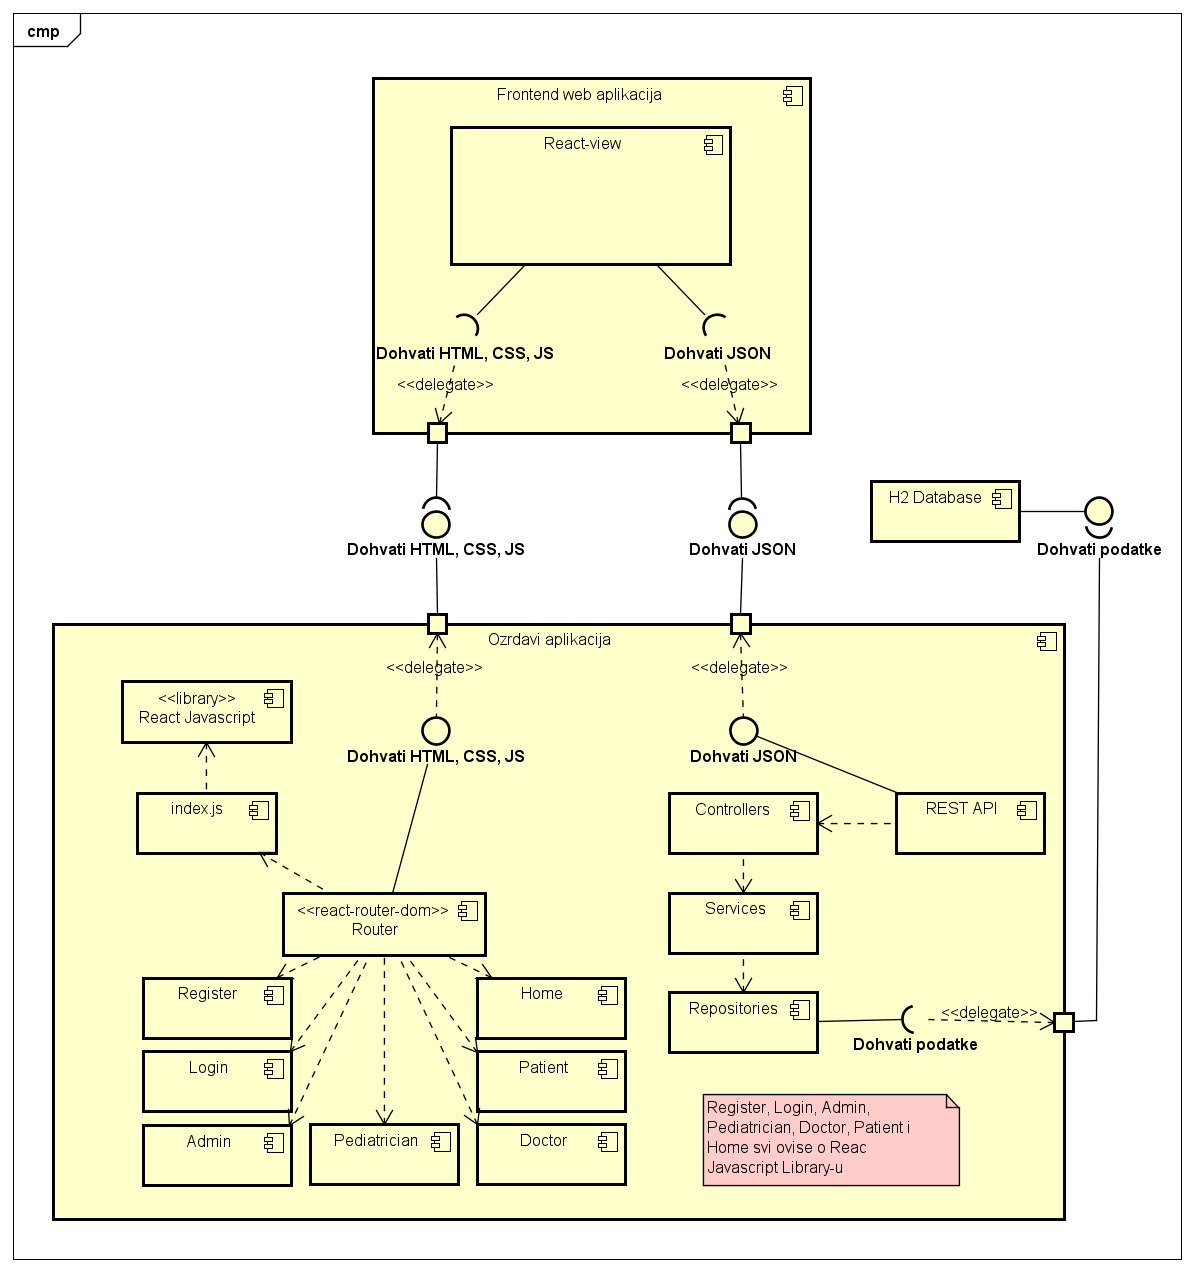
\includegraphics[scale=0.5]{dijagrami/dijkomp.PNG} %veličina slike u odnosu na originalnu datoteku i pozicija slike
				\centering
				\caption{Dijagram komponenti}
				\label{fig:dijkomp}
			\end{figure}
			